\section{Virtual Machines Preparation}

\centeredlargetext{white}{black}{
Virtual Machines Preparation II
}

\begin{frame}
\frametitle{Booting the Virtual Machine}
\begin{itemize}
\item Click on the ``ITKv4'' icon on the left, to select it.
\item Click on the Green Arrow at the top ``Show''.
\item The VM will start to boot and you will see the warning:
\end{itemize}
\begin{center}
  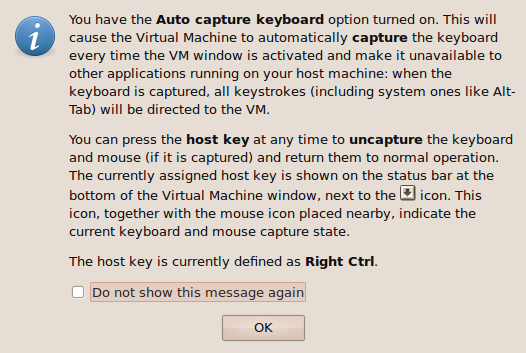
\includegraphics[width=0.4\paperwidth]{../Art/Screenshot-VirtualBox-OSE-02.png}
\end{center}
\begin{itemize}
\item Click ``OK''
\end{itemize}
\end{frame}

\begin{frame}
\frametitle{Booting the Virtual Machine}
\begin{itemize}
\item The boot sequence should continue and you shold see:
\end{itemize}
\begin{center}
  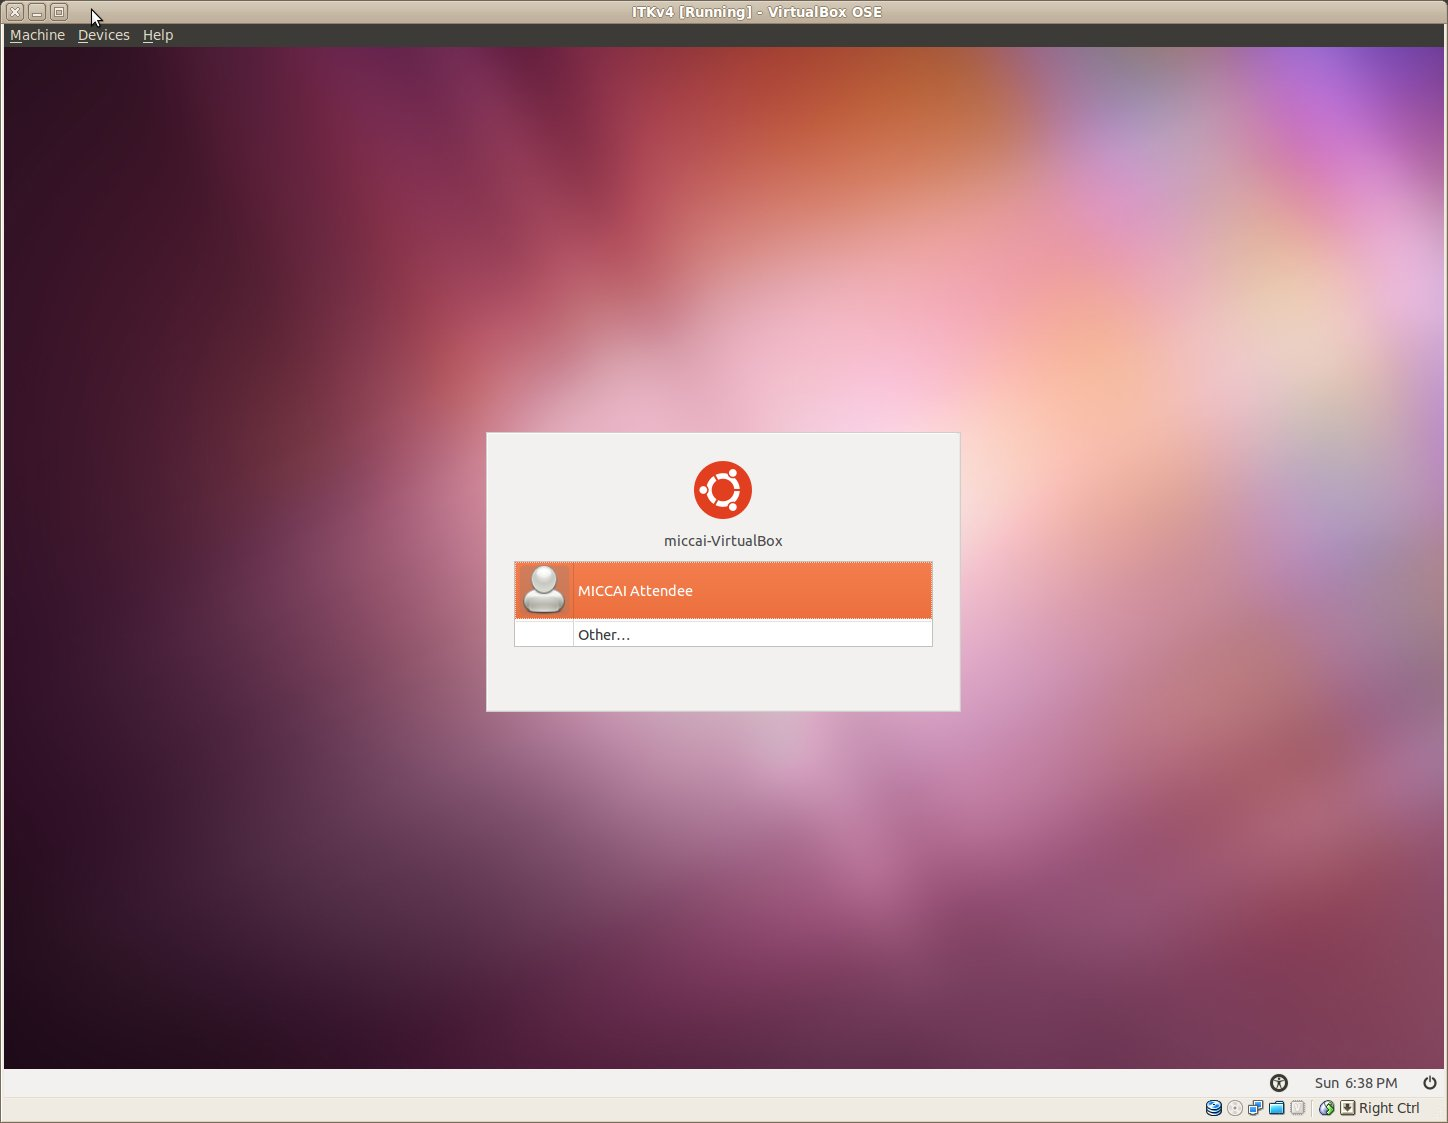
\includegraphics[width=0.7\paperwidth]{../Art/Screenshot-ITKv4-VirtualBox-01.jpg}
\end{center}
\begin{itemize}
\item Login with the password: ``toronto''
\end{itemize}
\end{frame}

\begin{frame}
\frametitle{Booting the Virtual Machine}
\begin{itemize}
\item After logging in you should see:
\end{itemize}
\begin{center}
  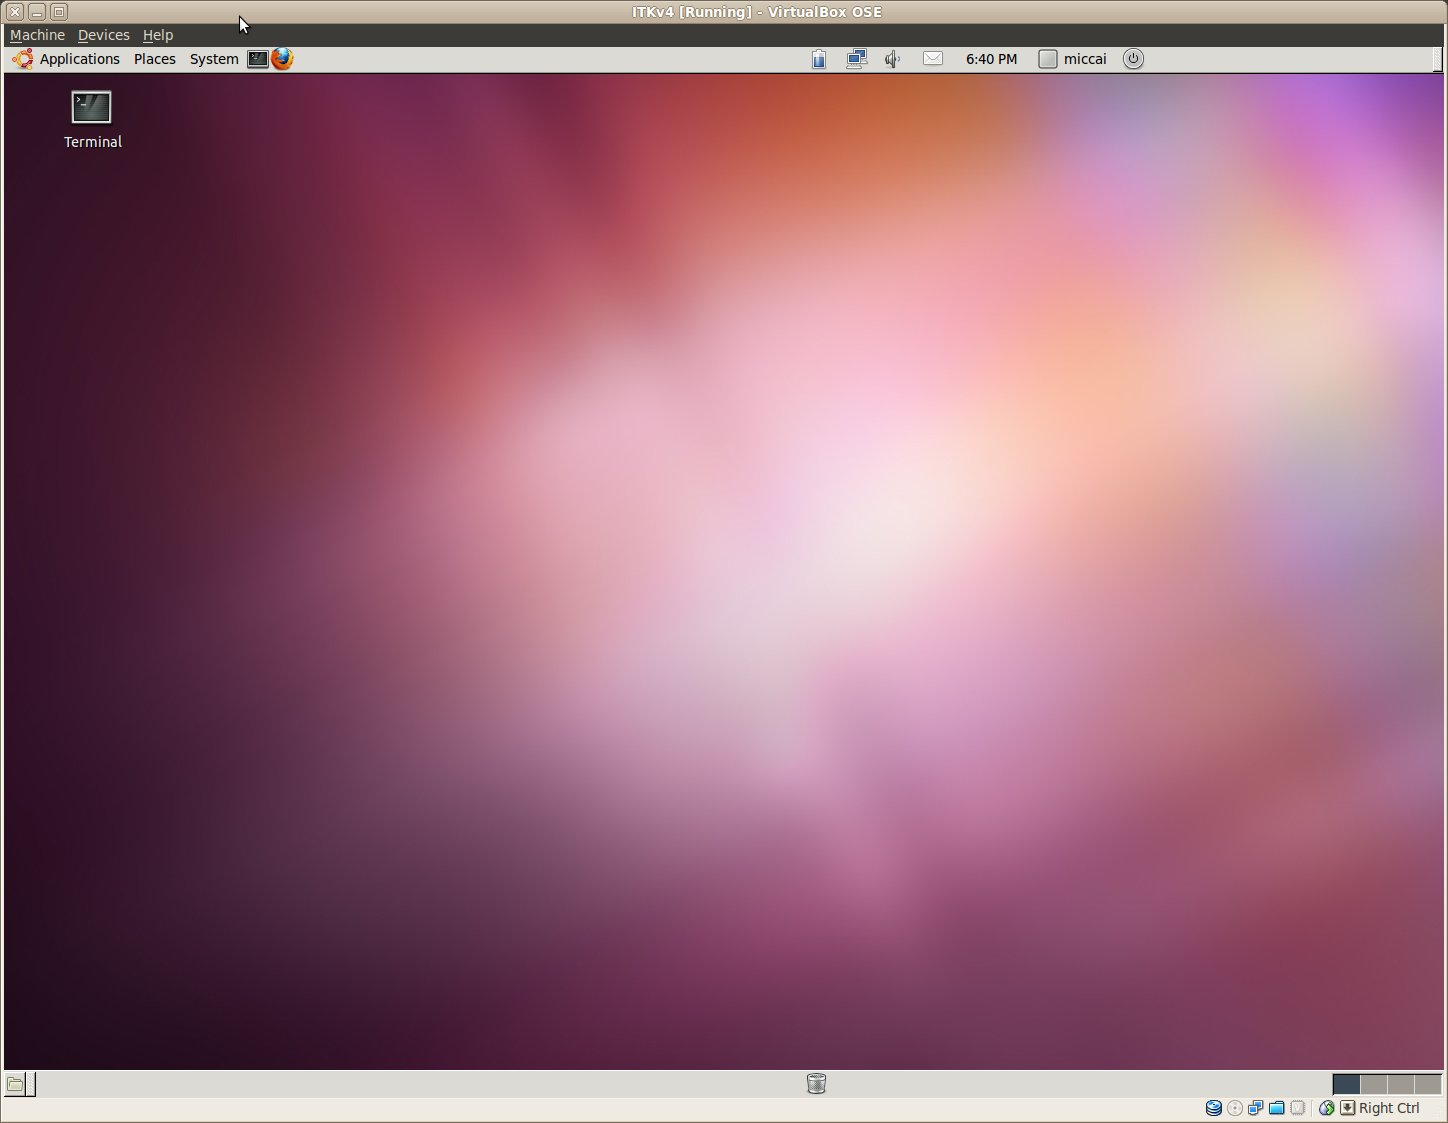
\includegraphics[width=0.7\paperwidth]{../Art/Screenshot-ITKv4-VirtualBox-02.jpg}
\end{center}
\end{frame}


\centeredlargetext{white}{black}{
Your Virtual Machine\\ is Ready !
}

\begin{frame}
\frametitle{Additional Copies}
\begin{itemize}
\item The same source trees are available in the DVD / USB key
\item Outside of the VirtualBox image
\end{itemize}
\end{frame}

